%----------------------------------------------------------------------------
\chapter{Összefoglalás, fejlesztési lehetőségek}\label{sect:Summary}
%----------------------------------------------------------------------------

\hspace{2mm} Elmondhatom, hogy a félév során rengeteget tanultam, megismerkedtem modern webfejlesztési eszközökkel és implementáltam egy kiterjedt osztályhierarchiával rendelkező komoly naptár kezeléssel bíró webes alkalmazást. Az alkalmazás kódja ennek a dokumentációnak a plain latex kódjával együtt megtalálható a Github Repository-mban \cite{TDoneRepo}  a webes applikációval együtt. \cite{TDoneWeb} Az applikáció képét mutatja \figref{App}-es ábra.

\begin{figure}[!ht]
\centering
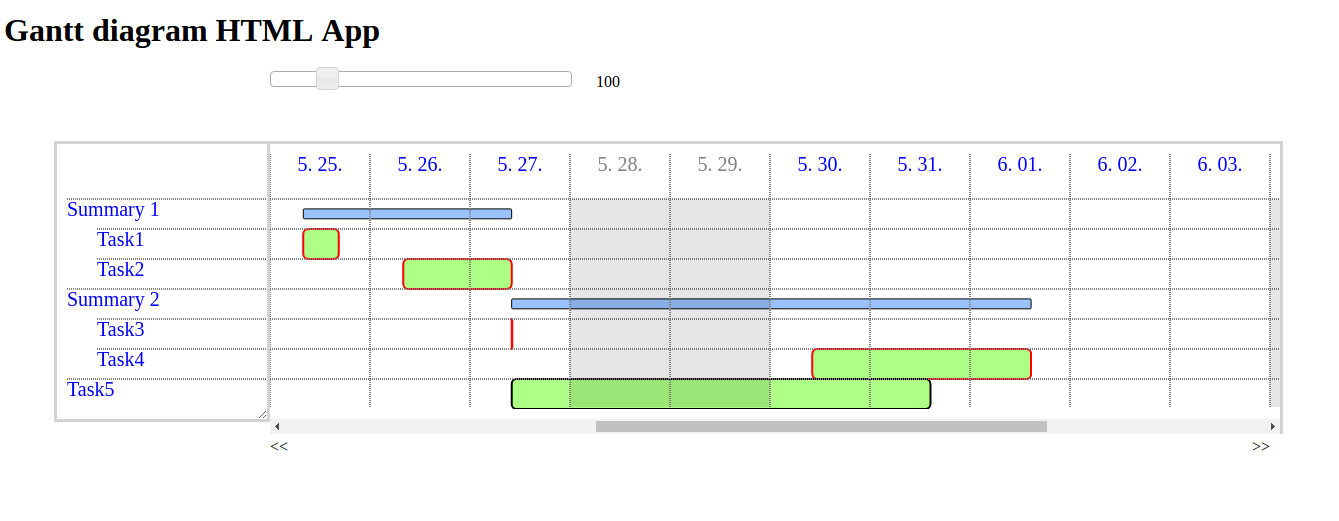
\includegraphics[width=\textwidth, keepaspectratio]{figures/application.png}
\caption{Az elkészített applikáció képe} 
\label{fig:App}
\end{figure} 

A projekten még rengeteget lehet fejleszteni. A teljesség igénye nélkül:
\begin{itemize}
\item Magának a weboldalnak a külalakjának fejlesztés (AngularJS)
\item Fájlkezelés megvalósítása
\item Bemenetei adatok megadhatósága a felületen
\item Input validáció
\item Diagram kinézetének fejlesztése
\end{itemize}